\documentclass[10pt]{beamer}

\usetheme{Montpellier}
\usecolortheme{whale}

\usepackage[T1]{fontenc}
\usepackage{lmodern}

\usepackage{mathtools}
\usepackage[binary-units]{siunitx}
\usepackage{amsmath}
\usepackage{listings}
\usepackage{mdframed}
\usepackage{adjustbox}
\usepackage{minted}
\usepackage{xcolor}

\usepackage{parskip}
\usepackage{substr}
\usepackage{hyperref}
\usepackage{etoolbox}
\usepackage{tipa}
\usepackage{cprotect}
\usepackage{booktabs}
\usepackage{silence}
\usepackage[backend=biber, style=ieee]{biblatex}
\usepackage[english,ngerman]{babel}
\usepackage{csquotes}

\definecolor{lg}{gray}{0.95}
\hypersetup{colorlinks = true, urlcolor=blue, linkcolor=white}
\WarningFilter{biblatex}{Patching footnotes failed}

\renewcommand*{\bibfont}{\tiny}
\renewcommand{\subsectionname}{AA}

\bibliography{resources.bib}

\title{\textbf{Operating Systems}}
\subtitle{Tutorial 10}
\author{Fabian Klopfer}
\date{\today}

\defbeamertemplate{subsection page}{mine}[1][]{%
    \begin{centering}
        {\usebeamerfont{subsection name}\usebeamercolor[fg]{subsection name}#1}
        \vskip1em\par
        \begin{beamercolorbox}[sep=12pt,center]{part title}
            \usebeamerfont{subsection title}\insertsubsection\par
        \end{beamercolorbox}
    \end{centering}
    }

    \defbeamertemplate{section page}{mine}[1][]{%
        \begin{centering}
            {\usebeamerfont{section name}\usebeamercolor[fg]{section name}#1}
            \vskip1em\par
            \begin{beamercolorbox}[sep=12pt,center]{part title}
                \usebeamerfont{section title}\insertsection\par
            \end{beamercolorbox}
        \end{centering}
        }

        \setbeamertemplate{section page}[mine]
        \setbeamertemplate{subsection page}[mine]

        \begin{document}
        \frame{\titlepage}

        \begin{frame}{Intro}
            \begin{itemize}
                \item Pingo Polls
                \item Solution sheet 8
                \item Preview sheet 9
            \end{itemize}
        \end{frame}

        \begin{frame}{\alert{Inofficial} exam-relevant exercises list}
            Union of tasks \& questions considered relevant by Max \& Fabian. \vspace{0.3cm} \\
            Official list/sample exam to follow soon. \vspace{0.5cm} \\
            Comprehension questions:
            \begin{itemize}
                \item 1.1.1, 1.1.3-4, 2.1.2-4, 2.1.6, 2.4.3-5, 2.4.7, 3.1.1, 3.1.3, 4.1.1-4, 4.1.7, 5.1.1-2, 5.1.4-9, 6.1.2, 6.1.4-8, 7.1.2, 7.1.5, 7.1.7
            \end{itemize}

            Exercises:
            \begin{itemize}
                \item 1.4, 2.2, 2.3, 3.3, 3.4, 4.3, 4.4, 4.5, 5.2, 5.3, 5.4, 5.5, 6.2, 6.3, 6.4, 6.5, 7.2, 7.3, 8.2, 8.3, 8.4
            \end{itemize}
        \end{frame}

        \section*{Exercise sheet 8}
        \frame{\sectionpage}
        \begin{frame}[allowframebreaks]{Exercise 1: Comprehension Questions}
            \begin{enumerate}
                \item Does active waiting work for cooperative scheduling? \\
                    \alert{No, as control has to be passed. \\
                    Cooperative scheduling + active waiting $\Rightarrow$ nothing else executes $\Rightarrow$ resources won't be released $\Rightarrow$ Deadlock}

                \item Does the solution with active waiting and \mintinline{c}{turn} variable in Figure~2.23 in \autocite{tanenbaum} with two CPUs and shared memory? \\
                    \alert{Yes, simply use one number per process (e.g. process 5 is allowed to run when \mintinline{c}{turn = 5}}

                \item Can the priority inversion problem occur with threads in user space? \\
                    \alert{Can only occur with preemptive scheduling. (No)}

                \item Can race conditions occur if all threads are executed on a single core? \\
                    \alert{Yes! When a thread/process gets interrupted and the next one uses the unfinished state \\  A wants to remove an element from the list and gets interrupted before decrementing the counter (e.g. length variable). \\
                    B wants to add something reads the wrong length and inserts at wrong position.}

                \item At an intersection, four cars are each waiting for the car to their right to enter the intersection. Is this a deadlock? \\
                    \alert{Obviously. Circular wait.}


                \item Under what circumstances can resource traces be diagonal? (Figure 6.8 in \autocite{tanenbaum}) \\
                    \alert{When enough resources are available such that there is a schedule where processes don't need to wait for resources to be released.}

                \item How can the scheme of resource trajectories (Figure~6.8 in \autocite{tanenbaum}) be extended to any number of processes? \\
                    \alert{One axis/dimension per process.}

                \item In a system with two processes and three instances of a resource, can there be a deadlock if each process requires two instances of the resource? Why? \\
                    \alert{No. One process gets two and executes, the other waits. When the former finishes the latter gets the resources and can execute.}
            \end{enumerate}
        \end{frame}

        \begin{frame}[allowframebreaks]{Exercise 2: Deadlocks}
            \begin{enumerate}
                \item The four criteria for deadlocks are {necessary} for deadlocks, but not {sufficient}. \\
                    Conditions:
                    \begin{itemize}
                        \item No Preemption
                        \item Hold and wait
                        \item Mutual Exclusion
                        \item Circular Wait
                    \end{itemize}
                    Give an example of a case that meets the four criteria but does not cause a deadlock. \\
                    \framebreak

                    \alert{Non-preemptive scheduling. Resources are thread safe using MutEx.\\
                    Processes A, B, C. \\
                    Resource types S (2 instances), R (1 instance). \\
                    A requests R, gets it \\
                    B requests S, gets it \\
                    C requests S, gets it \\
                    B requests R, blocked \\
                    A requests S, blocked \\
                    B waits for A, A waits for B (or C) $\Rightarrow$ Circular wait. 1-3 by assumption. \\
                    When C executes and releases it's instance of S, A can continue then B.}

                \item Specify a condition under which the four criteria are necessary and sufficient for deadlocks. \\
                    \alert{When resources are unique. There is no way to break the circular wait then.}
            \end{enumerate}
        \end{frame}

        \begin{frame}[allowframebreaks]{Exercise 3: Amdahl's Law}
            $T$: total execution time of program sequentially, \vspace{0.5cm} \\
            $B$: time to execute sequential parts, \vspace{0.5cm} \\
            $T-B$: time to execute parallel parts sequentially, \vspace{0.5cm} \\
            $N$: number of CPUs. \vspace{0.5cm} \\
            Total execution time on $N$ CPUs: $T(N) = B + (T - B) / N$. \vspace{0.5cm} \\
            Total speed-up $T / T(N)$. \vspace{0.5cm} \\
            Speed-up factor: $S = \frac{1}{B + (1 - B)/N}$ \vspace{0.5cm} \\
            \framebreak
            \begin{enumerate}
                \item A program's sequential part is $1\,\%$.
                    By what factor is the program accelerated when executed on $61$ CPUs? \\
                    \alert{$S =  1 / \bigl( 0.01 + (1 - 0.01) / 61 \bigr) = 38.125$.}

                \item To which value does the speed-up~$S$ converge for $N \rightarrow \infty$? \\
                    \alert{
                        \[ \lim_{N\rightarrow\infty} \frac{1}{B + (1-B)/N} = \frac{1}{B} \]
                    }

                \item Amdahl's rule does not take into account the cost of communication between CPUs.
                    Extend the expression for the speed-up~$S$ to include communication costs~$C$.
                    \alert{\[ S = \frac{1}{B + (1 - B)/N + C} \]
                    So What is C? Load balancing of scheduler, locking/waiting, message passing, ... }

                \item%
                    Two implementations of an algorithm have the same sequential fraction of $B=0.001$,
                    but differ in their communication costs of $C_1 = 0.0001 N$ and $C_2 = 0.001 \ln(N)$.
                    Determine the number of CPUs~$N$ with maximum speed-up~$S$ for both implementations. \\
                    Extremum is a $0$ of the derivative wrt. N, and minimize denominator to maximize: \\
                    \alert{First $C_1 = 0.0001$:
                    \[  \frac{\partial}{\partial N} B + (1-B) \cdot N^{-1} + 0.0001 N = 0 \]
                    \[-(1-B)N^{-2} + 0.0001 = 0  \]
                    \[ N^{-2} = \frac{0.0001}{1-B} \]
                    \[ N^{2} = 10000 \cdot (1-B) \]
                    \[ N = 100 \cdot \sqrt{1 - B} \]

                    Now for $C_2 = 0.001 \ln(N)$:
                    \[  \frac{\partial}{\partial N} B + (1-B) \cdot N^{-1} + 0.001 \ln{N} = 0 \]
                    \[-(1-B)N^{-2} + 0.001 N^{-1} = 0  \]
                    \[  1000 N = \frac{N^2}{1-B} \]
                    \[  (1 - B)(1000 N) = N^2 \]
                    \[  (1-B) = \frac{N}{1000} \]
                    \[ N = 1000 \cdot (1 - B) \]
                    $100$ and $1000$ depending on how much is parallelizable.}
                    \framebreak

                \item Plot the speed-up~$S$ as a function of the number of CPUs~$N$ for both algorithms and $1 \leq N \leq 1500$. \\
                    \begin{figure}
                        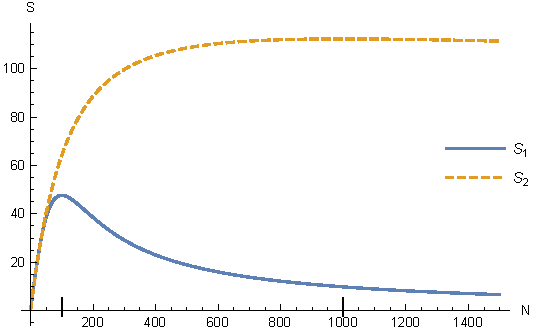
\includegraphics[keepaspectratio, width=0.8\textwidth, height=\textheight-2\baselineskip-2\baselineskip]{img/amdahl.pdf} \\
                    \end{figure}

                \item How do the two implementations differ qualitatively in the change in their speed-up when they use more CPUs than is optimal for them?
                    \alert{The larger the communication costs, the larger the penalty when using more CPUs.}
            \end{enumerate}
        \end{frame}



        \begin{frame}[allowframebreaks,fragile]{Exercise 4: Race Conditions}
            \begin{minipage}[t]{0.5\linewidth-\tabcolsep}
                What is the value of \mintinline{c}{total_count} (depending on~\mintinline{c}{n}) after a call to \mintinline{c}{total}? \\
                \alert{$0$} \vspace{0.5cm} \\

                The function \mintinline{c}{total} is executed in several threads simultaneously.
                Describe the race condition in the program snippet. Which variables are affected? What is the effect of the race condition?
            \end{minipage}%
            \hfill%
            \begin{minipage}[t]{0.5\linewidth-2\tabcolsep}
                \begin{minted}[autogobble]{c}
                    const int n = 5000;
                    int total_count;

                    void total(void)
                    {
                        int count = 0;
                        for (; count < n; ++count)
                        if (count % 2)
                        --total_count;
                        else
                        ++total_count;
                    }
                \end{minted}
            \end{minipage}
            \framebreak

            \begin{minipage}[t]{0.4\linewidth-\tabcolsep}
                \alert{Threads may read while another thread is in the write process. \\
                I.e. the thread changes the value in a register but hasn't stored the result back to memory \\
                Another thread reads the lower value and overwrites the result\\
                i.e. instead of 2 increments we only have one \\
                Possible values: $\pm \frac{n}{2} - 1 \cdot |threads|$}
            \end{minipage}%
            \hfill%
            \begin{minipage}[t]{0.5\linewidth-2\tabcolsep}
                \begin{minted}[autogobble]{c}
                    const int n = 5000;
                    int total_count;

                    void total(void)
                    {
                        int count = 0;
                        for (; count < n; ++count)
                        if (count % 2)
                        --total_count;
                        else
                        ++total_count;
                    }
                \end{minted}
            \end{minipage}
            \framebreak


            Fix the race condition by using a semaphore.
            To do this, you can use a semaphore \mintinline{c}{int semaphore;} and the functions \mintinline{c}{void up(*int)} and \mintinline{c}{void down(*int)}. \\
            \alert{Show code.}


        \end{frame}

        \section*{Exercise sheet 9}
        \frame{\sectionpage}
        \begin{frame}[allowframebreaks, fragile]{}
            \begin{figure}
                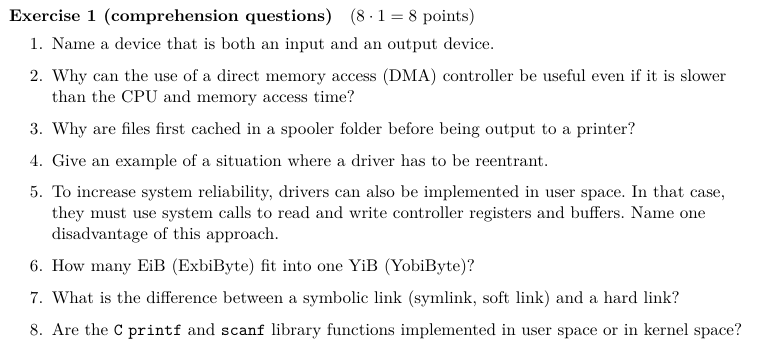
\includegraphics[keepaspectratio, width=\textwidth, height=\textheight-2\baselineskip-2\baselineskip]{img/ex9_100.png} \\
            \end{figure}
            \framebreak
            \begin{itemize}
                \item easy
                \item How fast are IO devices?
                \item Think about Deadlocks
                \item ex. many examples
                \item Mode switch vs. memory access
                \item do the math
                \item Think of the Inode level? What does a symlink do? What does a hard link do? (shallow vs deep copy)
                \item Is the C library (glibc or libc) part of the kernel?
            \end{itemize}
            \framebreak

            \begin{figure}
                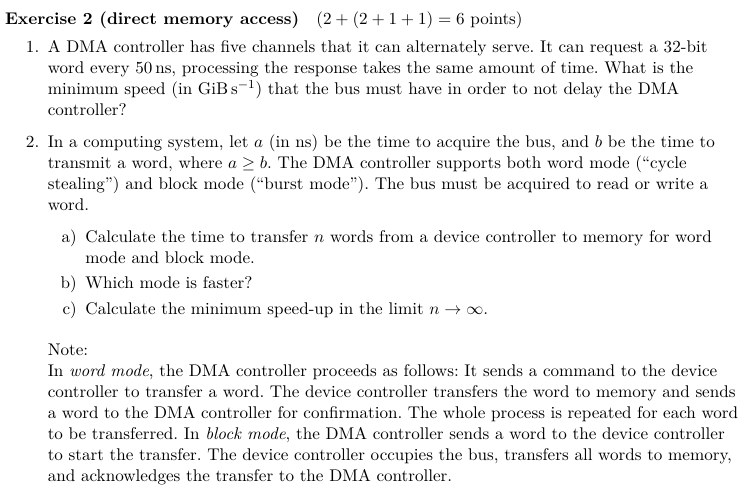
\includegraphics[keepaspectratio, width=\textwidth, height=\textheight-2\baselineskip-2\baselineskip]{img/ex9_101.png} \\
            \end{figure}
            \framebreak
            \begin{itemize}
                \item  word size / latency = bit/ns
                \item command to + read from + write to for word mode. \\
                    command to + reserve once, n reads + ack
                \item trivial
                \item fraction of the fromulas from a with n to infinity.
            \end{itemize}
            \framebreak

            \begin{figure}
                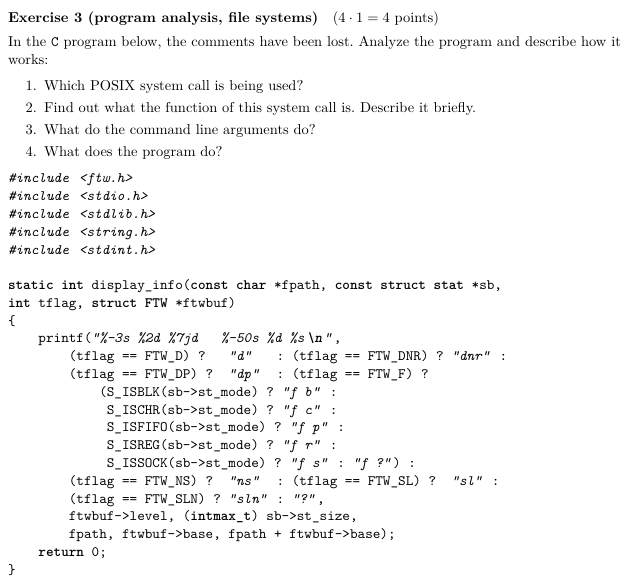
\includegraphics[keepaspectratio, width=\textwidth, height=\textheight-2\baselineskip-2\baselineskip]{img/ex9_102.png} \\
            \end{figure}
            \framebreak
            \begin{itemize}
                \item A large printf with nested if statements
                \item what do the flags and constants mean? Look for the documentation
                \item What are the arguments? What is the \mintinline{c}{stat} struct?
                \item What is ftw.h for?
            \end{itemize}
            \framebreak
            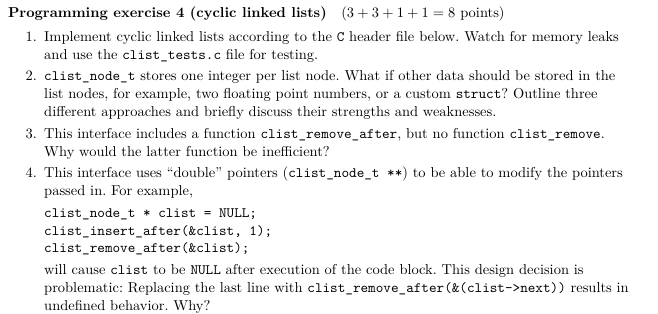
\includegraphics[keepaspectratio, width=\textwidth, height=\textheight]{img/ex9_103_0.png} \\
            \begin{itemize}
                \item Remember KDI. Make the next pointer of the tail point to the header.
                \item you only need to insert and remove directly after the head (i.e. at one place)
                \item Use the address sanitizer.
            \end{itemize}
            \framebreak
            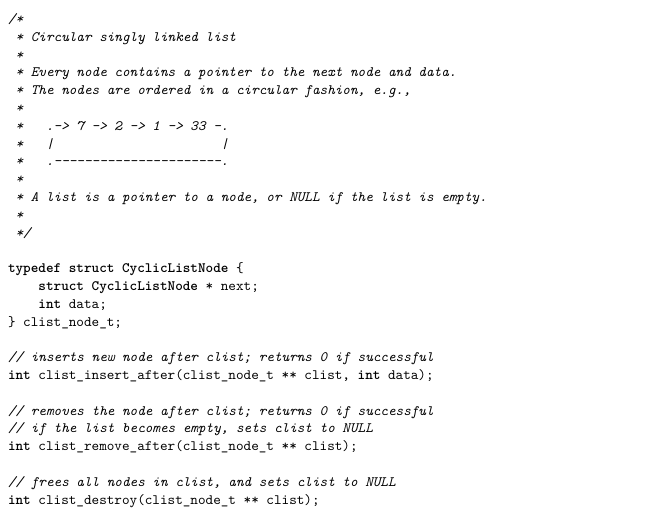
\includegraphics[keepaspectratio, width=0.69\textwidth, height=\textheight]{img/ex9_103_1.png}
            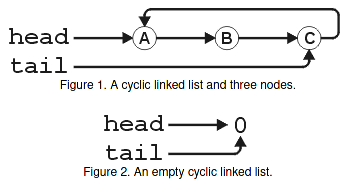
\includegraphics[keepaspectratio, width=0.3\textwidth, height=\textheight]{img/cyc.png} \\

        \end{frame}

        \section{References}
        \begin{frame}[allowframebreaks]
            \frametitle{References}
            \begin{tiny}
                \nocite{*}
                \printbibliography
            \end{tiny}
        \end{frame}


    \end{document}

